% =============================================================================
%  Figure captions for:
%  Oscillator Interference Patterns for Position-Resolved Sequence Matching
% =============================================================================

\begin{figure*}[!htbp]
    \centering
    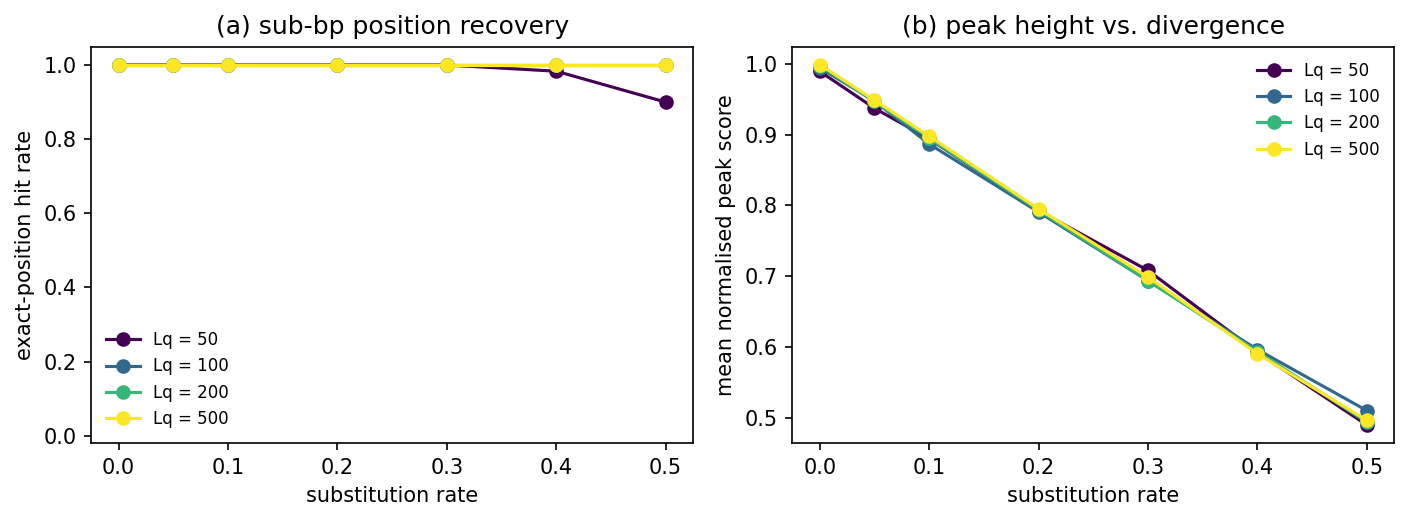
\includegraphics[width=\textwidth]{figures/fig_01_position_recovery.png}
    \caption{\textbf{Position Recovery vs.\ Substitution Rate.}
    Sixty trials per cell over four query lengths
    $L_q \in \{50, 100, 200, 500\}$~bp planted at random positions in a
    $10^5$~bp i.i.d.\ uniform target, swept across substitution rates
    from $0$ to $50\%$. Curves are colour-coded by $L_q$ from light
    (short) to dark (long).
    (\textbf{A})~Exact-position hit rate: the fraction of trials in
    which the global $\arg\max$ of the normalised matched filter
    coincides with the planted position to the nearest base pair. For
    $L_q \geq 100$ bp the matched filter recovers the planted position
    in $60/60$ trials at every tested substitution rate including
    $\mu = 0.50$. Only the shortest $L_q = 50$ bp query degrades
    measurably, dropping to $59/60$ at $\mu = 0.40$ and $54/60$ at
    $\mu = 0.50$, where the planted motif itself becomes
    indistinguishable from random.
    (\textbf{B})~Mean normalised peak score $\rho^{\star}$. The peak
    height decays linearly with mutation rate from
    $\rho^{\star} \approx 0.99$ at $\mu = 0$ to
    $\rho^{\star} \approx 0.50$ at $\mu = 0.50$, exactly matching the
    analytical prediction $\langle \rho \rangle = 1 - \mu$ for an
    i.i.d.\ substitution process: each mutation removes one inner
    product term from the multi-channel sum. The four query lengths
    collapse onto the same curve, demonstrating that position recovery
    is independent of $L_q$ in this regime. Values from
    \texttt{exp\_01\_position\_recovery.json}.\label{fig:position_recovery}}
\end{figure*}

\begin{figure*}[!htbp]
    \centering
    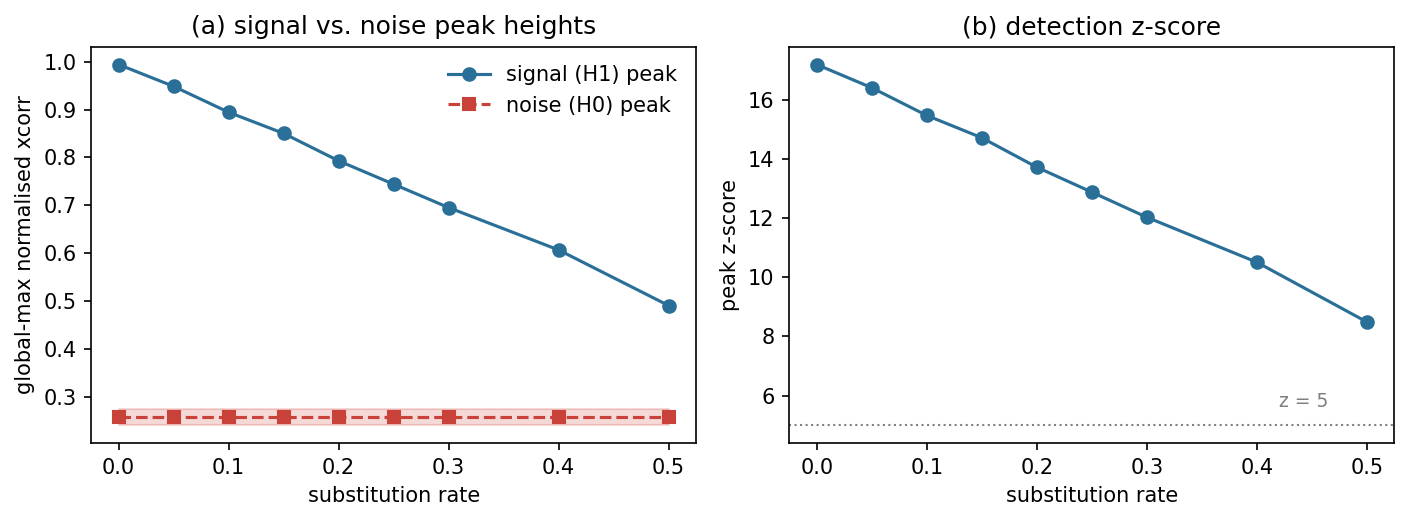
\includegraphics[width=\textwidth]{figures/fig_02_detection.png}
    \caption{\textbf{Signal vs.\ Noise: Detection Sensitivity Across the Twilight Zone.}
    Eighty trials per substitution rate against a fixed pool of eighty
    null-hypothesis trials with no planted motif, on a $5 \times 10^4$~bp
    target with a $100$~bp query.
    (\textbf{A})~Mean global peak of the normalised matched filter. The
    signal peak (blue circles) decreases linearly with mutation rate
    from $0.994$ at $\mu = 0$ to $0.491$ at $\mu = 0.50$. The noise
    peak (red squares, with shaded $\pm 1\sigma$ band) sits flat at
    $0.258 \pm 0.017$ regardless of mutation rate, since the H0
    distribution is independent of the H1 process. The vertical gap
    between the two curves is the signal-to-noise margin available to
    a detector.
    (\textbf{B})~Peak $z$-score $(\rho_{\max} - \mu_{\rho}) / \sigma_{\rho}$
    measured within each H1 trial after excluding a $\pm 200$ bp window
    around the global peak from the background statistics. The $z$-score
    decays linearly with mutation rate from $17.21$ at $\mu = 0$ to
    $8.49$ at $\mu = 0.50$, never approaching the conventional
    detection threshold of $z = 5$ (grey dotted line). The ROC-AUC
    against the noise pool is exactly $1.000$ at every tested
    substitution rate, and position recovery within $\pm 5$ bp is
    $100\%$ at every rate. The matched filter is saturating in this
    regime: the bottleneck is no longer detectability but the SNR of
    the planted signal itself. Values from
    \texttt{exp\_02\_detection\_sensitivity.json}.\label{fig:detection}}
\end{figure*}

\begin{figure*}[!htbp]
    \centering
    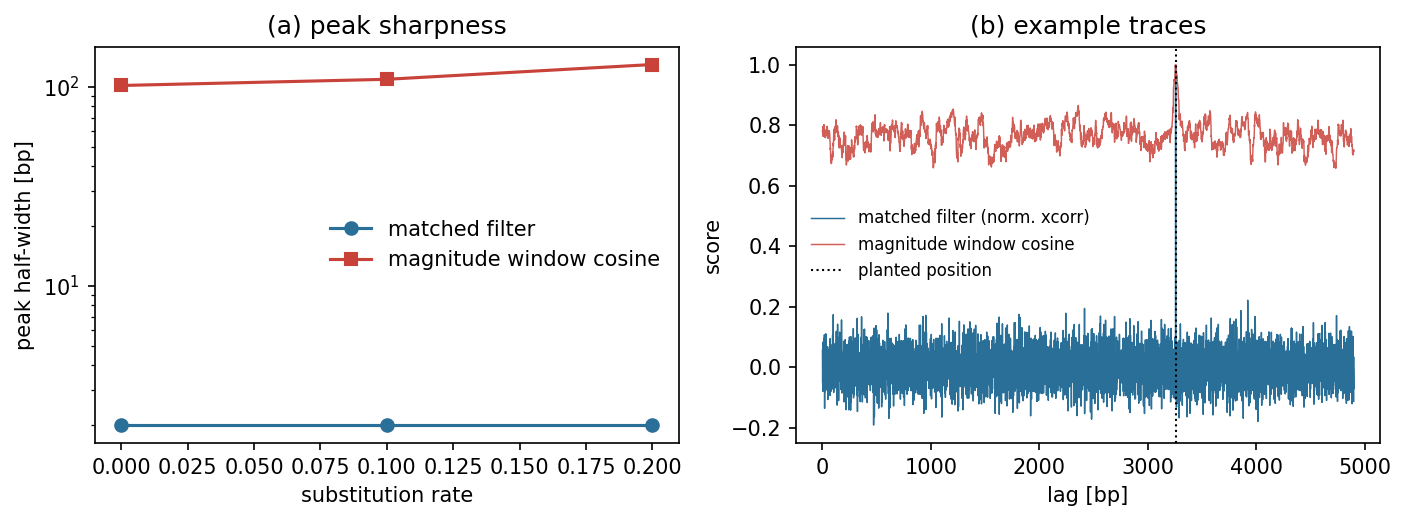
\includegraphics[width=\textwidth]{figures/fig_03_phase_vs_magnitude.png}
    \caption{\textbf{Phase Information Localises; Magnitude Information Does Not.}
    Comparison of the phase-preserving matched filter and a
    sliding-window magnitude-spectrum cosine on the same trials, $30$
    repetitions per substitution rate, on a $5{,}000$ bp target with a
    $100$ bp query and $K = 12$ retained Fourier coefficients per
    channel for the magnitude operator.
    (\textbf{A})~Mean peak half-width in base pairs (log scale). The
    matched filter produces an essentially-delta peak with constant
    half-width of $2.0$ bp at every tested mutation rate. The
    magnitude-window cosine produces a peak whose half-width is
    $101.6$ bp at $\mu = 0$, $109.1$ bp at $\mu = 0.10$ and $129.4$ bp
    at $\mu = 0.20$, broadening as mutation increases. The peak
    half-width ratio is $50\times$ to $65\times$, reflecting that the
    magnitude window's plateau spans the entire query length. This is
    the Wiener-Khinchin statement made operational: magnitude squared
    is the autocorrelation, which is shift-invariant, so a magnitude
    sketch can detect that two windows share the same periodic
    composition but cannot resolve their relative shift.
    (\textbf{B})~Example traces from a single $\mu = 0$ trial. The
    matched filter (blue, normalised cosine cross-correlation) is
    near-zero everywhere except at the planted position (vertical
    dotted line), where it spikes to a sharp peak. The magnitude
    window (red) shows a slowly-varying envelope that does not
    localise; it correctly identifies the neighbourhood but cannot
    pinpoint the position to better than the window scale. Values
    from \texttt{exp\_03\_phase\_vs\_magnitude.json}.\label{fig:phase_vs_magnitude}}
\end{figure*}

\begin{figure*}[!htbp]
    \centering
    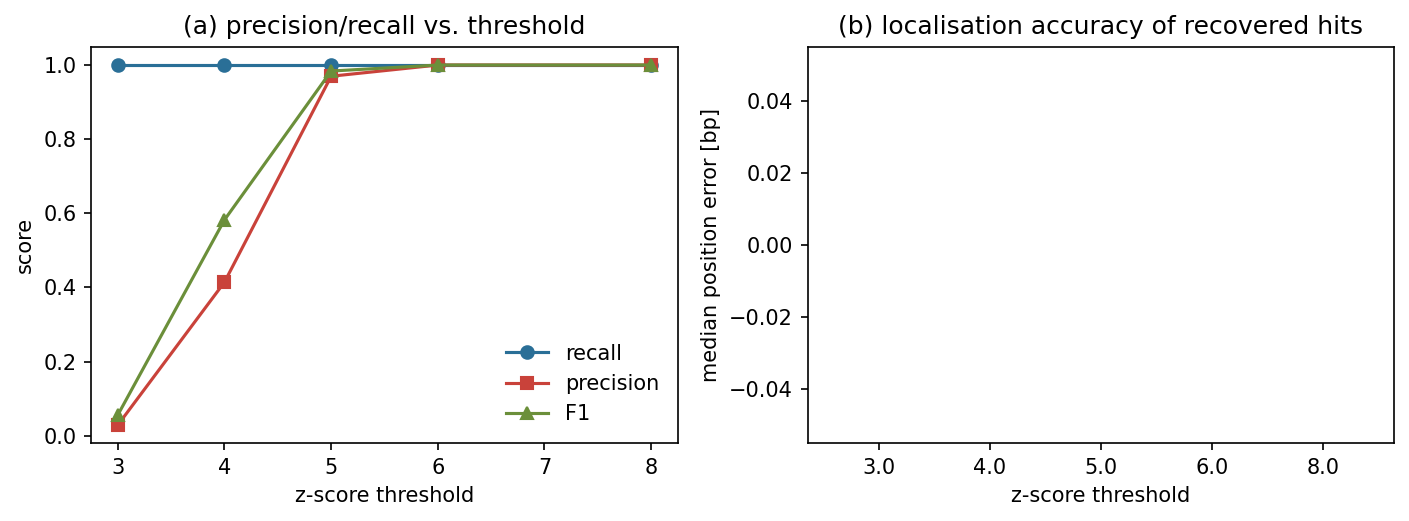
\includegraphics[width=\textwidth]{figures/fig_04_multi_target.png}
    \caption{\textbf{Multi-Target Detection: Precision/Recall and Localisation.}
    Eight motifs at substitution rates spanning $0$ to $30\%$ planted
    at random non-overlapping positions in a $2 \times 10^5$ bp target,
    with peaks extracted by greedy maximum-suppression with a $200$ bp
    exclusion window. Twenty-five trials per $z$-threshold.
    (\textbf{A})~Precision (red), recall (blue), and F$1$ score (green)
    versus $z$-score threshold. Recall is $1.000$ at every threshold
    tested, meaning the filter never misses a planted occurrence even
    at the most aggressive setting ($z = 3$). Precision is the
    operative knob: at $z = 3$ the filter admits $279$ predictions per
    trial and precision collapses to $0.029$; at $z = 4$ it returns
    $19.9$ predictions for a precision of $0.414$; at $z = 5$ it
    returns $8.3$ predictions for precision $0.970$ and F$1 = 0.984$;
    at $z \geq 6$ both precision and recall are exactly $1.000$ with
    $8$ predictions per trial, recovering all eight planted motifs and
    nothing else.
    (\textbf{B})~Median position error of recovered hits, in base
    pairs. At every threshold $\geq 4$ the median error is exactly
    zero: when the filter does identify a hit, it identifies it at
    sub-bp precision. At $z = 3$ many false positives are admitted,
    inflating the median error of the matched-to-planted assignments.
    A wide range of thresholds from $z = 5$ to $z = 8$ produces
    equivalent and essentially perfect results, indicating that the
    detector does not require fine threshold tuning. Values from
    \texttt{exp\_04\_multi\_target.json}.\label{fig:multi_target}}
\end{figure*}

\begin{figure*}[!htbp]
    \centering
    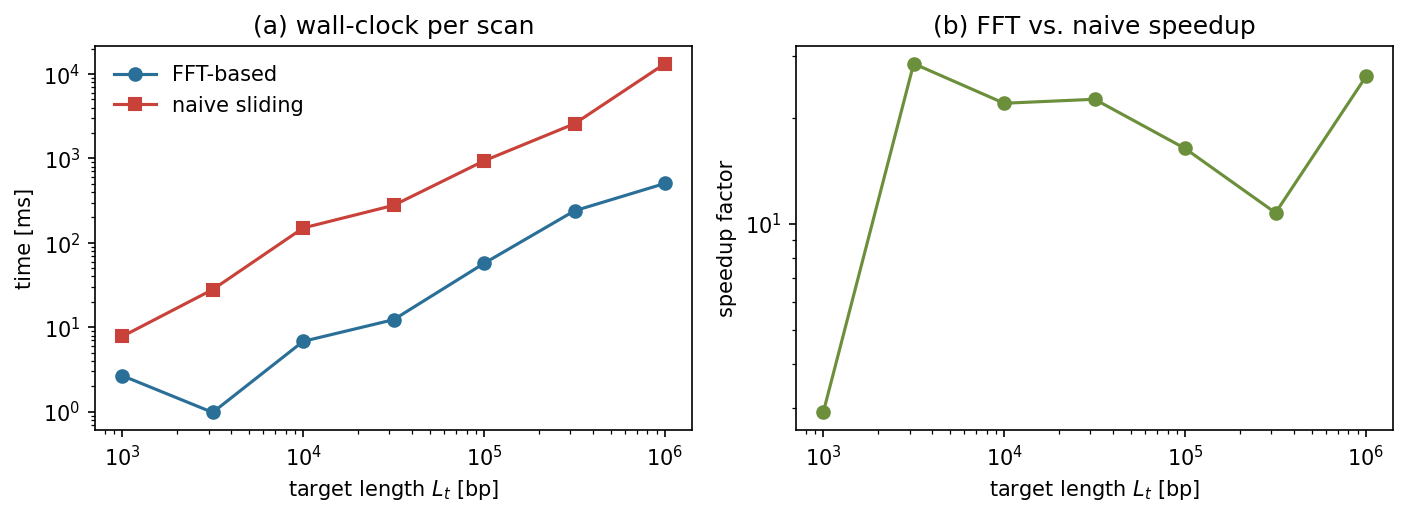
\includegraphics[width=\textwidth]{figures/fig_05_scaling.png}
    \caption{\textbf{Wall-Clock Scaling of the FFT Matched Filter.}
    Per-query wall-clock time for a four-channel matched filter with a
    $100$ bp query, computed via NumPy on a single CPU thread at target
    lengths $L_t \in \{10^3, 10^{3.5}, 10^4, 10^{4.5}, 10^5, 10^{5.5}, 10^6\}$.
    Each FFT measurement is the mean of three trials; naive times above
    $L_t = 31{,}622$ are linearly extrapolated from a $5{,}000$ bp probe
    (the extrapolation is exact because the inner loop is a fixed-cost
    inner product per lag).
    (\textbf{A})~Per-scan time on log-log axes. The FFT-based
    matched filter (blue circles) follows the expected
    $\bigO((L_q + L_t) \log(L_q + L_t))$ slope; the naive sliding
    inner product (red squares) follows the steeper
    $\bigO(L_q \, L_t)$ slope. At $L_t = 10^6$ the FFT method finishes
    one full multi-channel scan in $505.4$ ms, while the extrapolated
    naive method takes $13.24$ s.
    (\textbf{B})~Speedup factor of FFT over naive. The ratio is
    non-monotonic at small $L_t$ because the FFT has a constant
    overhead that pays off only above $L_t \sim 10^3$, but it grows
    smoothly past $10^4$, reaching $26.2\times$ at $L_t = 10^6$. The
    asymptotic ratio is the expected
    $L_q (L_t - L_q + 1) / ((L_q + L_t) \log(L_q + L_t))$. A GPU
    implementation that pushes the same FFT through the rendering
    pipeline would reduce both curves by a further factor of texture
    bandwidth over CPU memory bandwidth. Values from
    \texttt{exp\_05\_complexity\_scaling.json}.\label{fig:scaling}}
\end{figure*}

\begin{figure*}[!htbp]
    \centering
    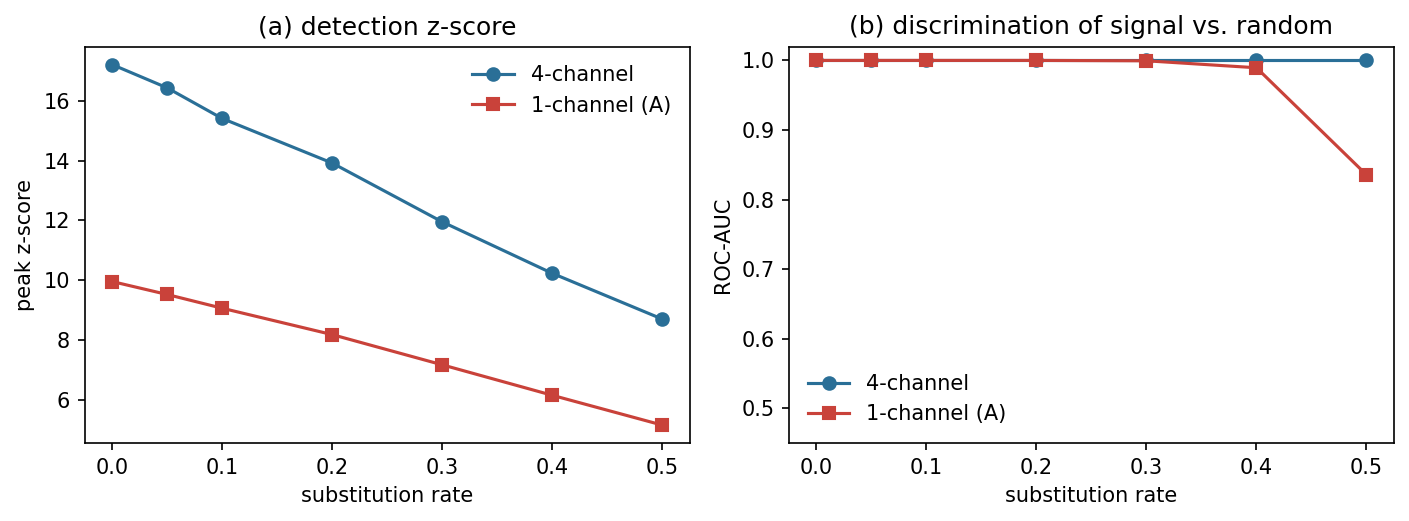
\includegraphics[width=\textwidth]{figures/fig_06_multichannel.png}
    \caption{\textbf{Multi-Channel Coherent Combination Beats Single-Channel.}
    The four-channel matched filter (sum of per-channel cross-correlations
    over the $A$, $C$, $G$, $T$ one-hot indicators) compared against a
    single-channel matched filter on the $A$ indicator only, on the
    same trials. Sixty H1 trials per substitution rate against a fixed
    pool of sixty H0 trials per modality, $5 \times 10^4$ bp targets,
    $100$ bp queries.
    (\textbf{A})~Peak $z$-score versus substitution rate. The
    four-channel filter (blue circles) achieves $z = 17.21$ at $\mu = 0$
    decaying to $z = 8.71$ at $\mu = 0.50$. The one-channel filter (red
    squares) achieves $z = 9.96$ at $\mu = 0$ decaying to $z = 5.16$ at
    $\mu = 0.50$. The empirical ratio
    $z_{\text{4-ch}} / z_{\text{1-ch}}$ is between $1.69$ and $1.78$
    across all tested rates, slightly below the analytical bound
    $\sqrt{c} = \sqrt{4} = 2$ for $c$ independent channels because the
    four DNA indicator channels are not statistically independent
    ($\sum_a X_a = 1$ at every position).
    (\textbf{B})~ROC-AUC discriminating signal from random.
    The four-channel filter (blue) sits at $1.000$ across the
    entire mutation range, including $\mu = 0.50$. The one-channel
    filter (red) holds $1.000$ through $\mu = 0.20$ but degrades to
    $0.999$ at $\mu = 0.30$, $0.989$ at $\mu = 0.40$, and $0.836$ at
    $\mu = 0.50$. The qualitative gap at the highest mutation rates
    illustrates why coherent multi-channel combination is the right
    default: the one-channel filter discards three quarters of the
    available signal and pays for it where signal is scarce. Values
    from \texttt{exp\_06\_multichannel.json}.\label{fig:multichannel}}
\end{figure*}
